\chapter{Clustering of CO emitters}

% Remove this first part.
Wide ASPECS' well-defined, large cosmic volume allows for some of the first direct constraints on the clustering of CO emitters.

Galaxies are not distributed entirely randomly in the universe. On the largest scales, the universe is isotropic and homogeneous, but on smaller scales, galaxies tend to cluster in space. One way to quantify how densely packed a population of galaxies is to compute the so-called two-point correlation function. This allows for the measuring of the mass of the dark matter halos in which these galaxies reside \cite{hickox2011clustering}. For a certain redshift, the more clustered a population of galaxies are, the more massive the halo that they are in.

The clustering of different populations of galaxies has been constrained by previous works, some of which is summarized in Fig. \ref{fig:Hickox_compare}, where the correlation length parameter, r0, which is a proxy for the amplitude of the clustering, is shown as a function of redshift for different populations. For example, \cite{hickox2011clustering} looked at the clustering of unobscured quasars and obscured quasars. \cite{10.1111/j.1365-2966.2011.20303.x} looks at the clustering in SMGs and compares their clustering to clustering found for other sets of astronomical objects, as can be seen in Fig. \ref{fig:Hickox_compare}. \cite{hickox2011clustering} found, in the Bo\"otes field, an $r_0$ for unobscured quasars to be $5.6 \pm 0.8$ at 0<z<1 and $r_0$ = [ADD], and for obscured quasars $6.0 \pm 1.0 $. In \cite{10.1111/j.1365-2966.2011.20303.x}, SMGs in the Extended Chandra Deep Field South were found to have a $r_0$ of $7.7_{-2.3}^{+1.8}$.

\begin{figure}[!htb]
\centering 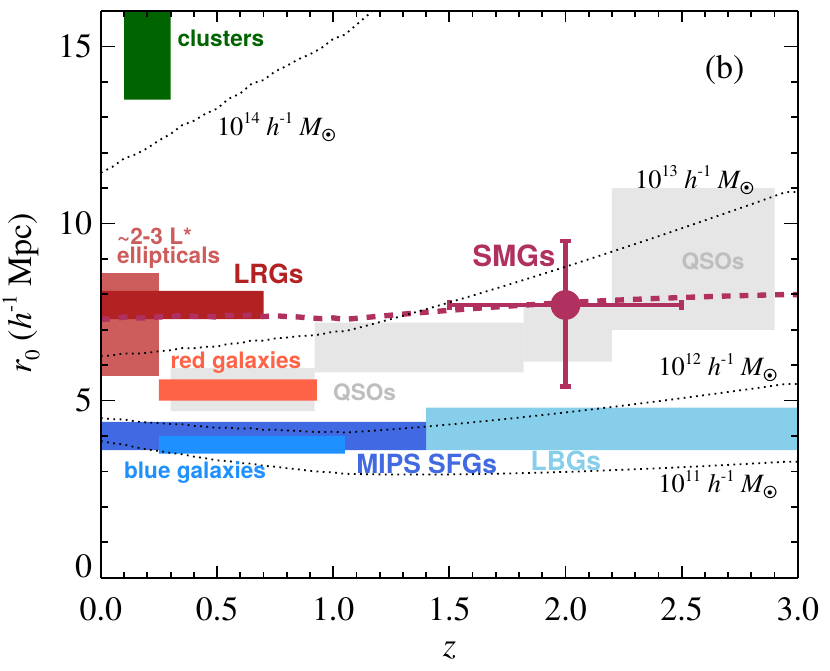
\includegraphics[width=87mm]{clustering/Hickox2012_Compare.png}
\caption{$r_0$ values for a variety of celestial objects as a function of redshift. The grey dotted lines show the evolution of $r_0$ for dark matter haloes of different masses. Figure adapted from \cite{10.1111/j.1365-2966.2011.20303.x}.}
\label{fig:Hickox_compare}
\end{figure}

\section{Method}

The clustering is computed through a two point correlation function. %The first step s to calculate the angular correlation function $ \omega(\theta)$. Once $ \omega(\theta)$ is computed, the second step is to obtain the two-point correlation function parameters of $r_0$ and $\gamma$.

The two-point correlation function, $ \xi(r)$ is the the probability of finding a galaxy at a separation $r$ from another randomly chosen galaxy in a volume $dV$ above Poisson, such that $$ dP = n(1 + \xi(r))dV $$, where $n$ is the mean space density of the galaxies in the universe\cite{hickox2011clustering}, and $\xi(r)$ is normally modeled as a power-law such that $\xi(r)$ = $(\frac{r}{r_0})^{-\gamma}$. In practice, the 3D separation $r$ between objects is hard to measure, then projected separations ($R$) or angular separations ($\theta$) are instead used. Here, we focus in the computation of the angular auto-correlation function $\omega(\theta)$. This quantity can be computed using the estimator from \cite{1993ApJ...412...64L} is used, where $$ \omega(\theta) = \frac{1}{RR}(DD-2DR + RR)$$, where $DD$, $DR$, and $RR$ are the number of data-data, data-random, and random-random galaxy pairs at a separation $\theta$, where each of the three collections is normalized to sum to 1 \cite{hickox2011clustering}. Here the 'data' catalog is represented by our actual CO emitter catalog, while the 'random' catalog is created by randomly distributing 20000 sources over the geometry of our survey, mimics exactly the same area where CO emitters were detected. The distribution of data and random sources are shown in Fig. \ref{fig:Clustering_points}.

%I think you are mixing a bit the things here. All the things about the fitting and getting r0 and gamma, z distribution, should be explained after to show all your clustering measurements.

%Then here
%1. first put that you checked your code using 2 random catalogs as you wrote below. And show the figure.

In order to check our code for the clustering computation, we created 2 additional random catalogs, of 20000 points each, and their angular correlation computed to show that it is consistent with zero, shown in Fig.\ref{fig:random_points}.

\begin{figure}[tbp]
[CHANGE TO ONE NEEDED -> FLAT ONE]
\centering 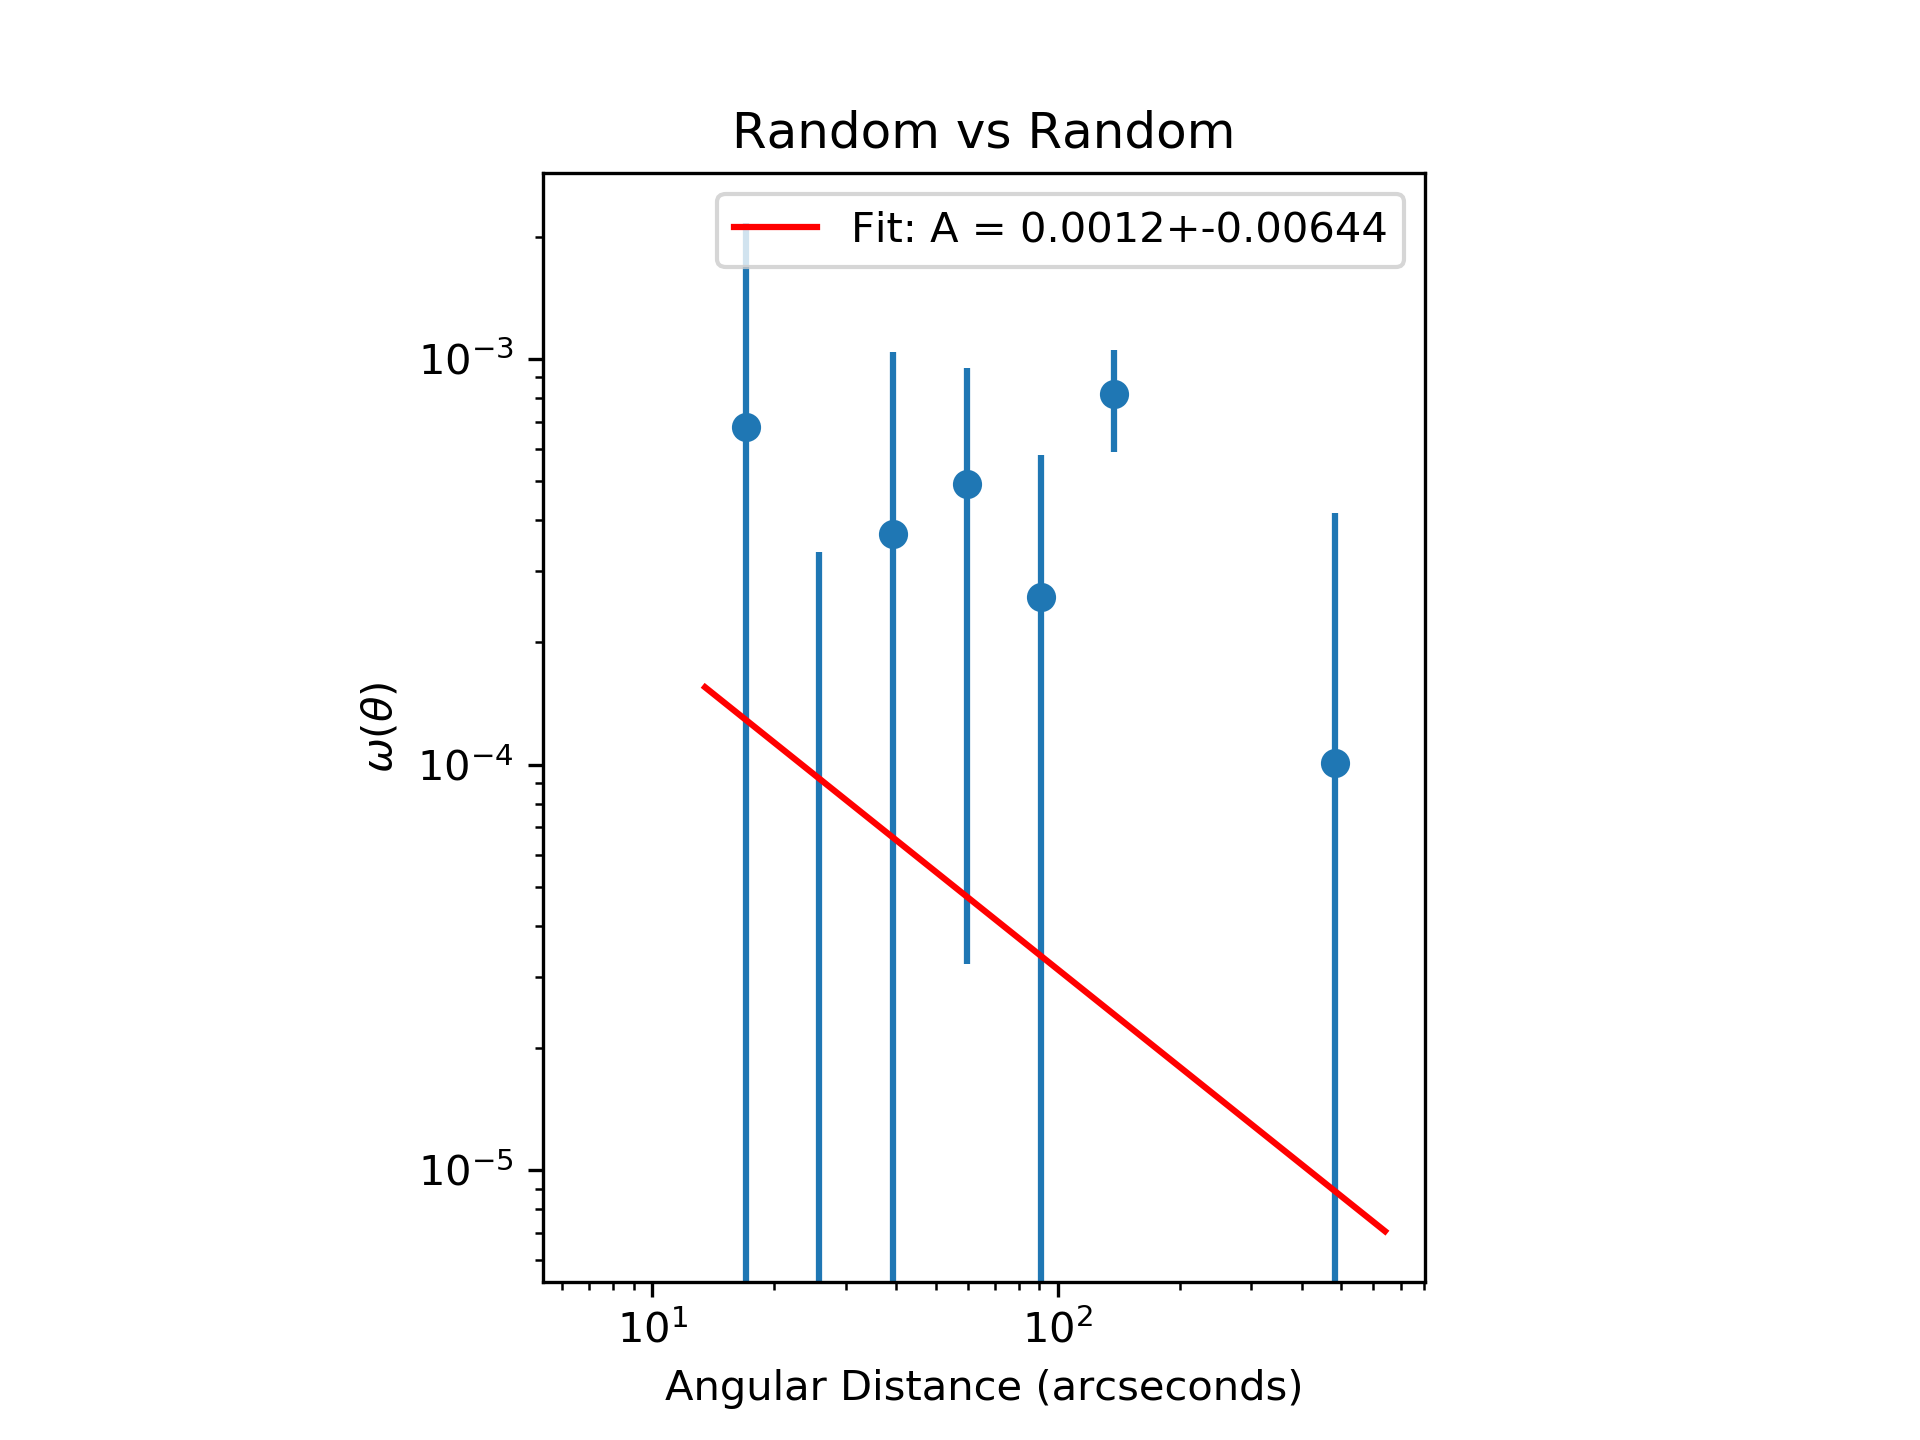
\includegraphics[width=100mm]{clustering/Log_Random_vs_Random_15000NoParenFlip_bin10.png}
\caption{Angular correlation two sets of random points used in this analysis, showing that the angular correlation is consistent with zero, as would be expected for cross-correlating two sets of uniformly distributed points.}
\label{fig:random_points}
\end{figure}


%2. put that you use your CO catalog (with fidelity >0.6) and the random catalog, and show your figure 3.5. Mention that you cut in z (put the redshift range used), Mention that you measured this in logaritmically spaced bins and put those numbers, and that you defined your lower bin as the minimum distance between objects in the catalog (although in your plot it looks like you are not doing that).

For this analysis, all CO line candidates above the 0.6 fidelity threshold were used, resulting in 35 sources, shown in Fig. \ref{fig:Clustering_points}. 

\begin{figure}[tbp]
\centering 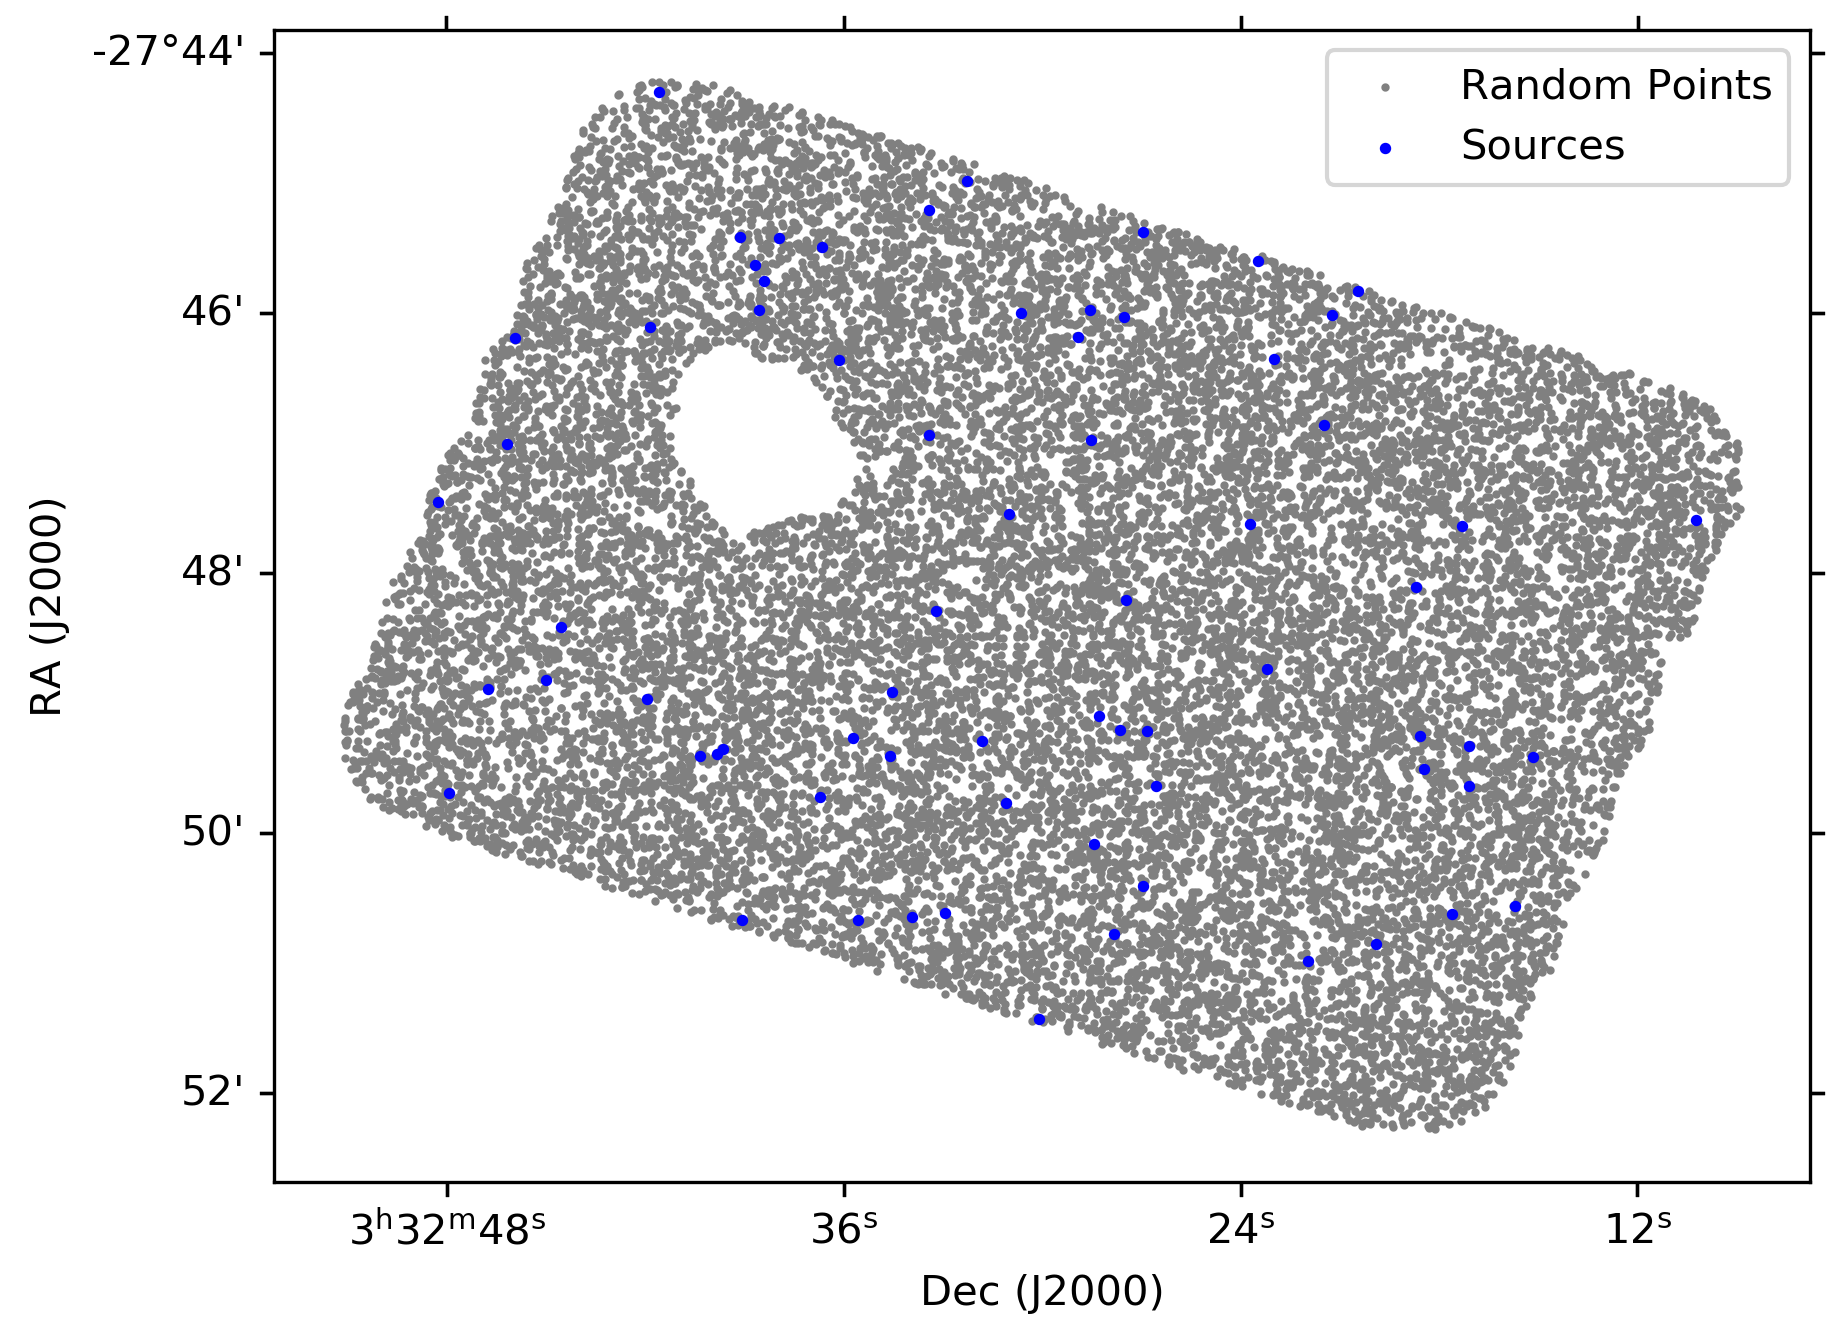
\includegraphics[width=120mm]{PDFS/NX_V_Y_Sources_20000.png}
\caption{Random points and sources from the $>$ 0.6 fidelity cut. The random points are distributed uniformly throughout the Wide ASPECS footprint.}
\label{fig:Clustering_points}
\end{figure}

\begin{figure}[!tbp]
% explain how bins can be negative and what this means for fitting only positive bins
% Bins can be negative through.... 0, so not negative I guess? 
\centering 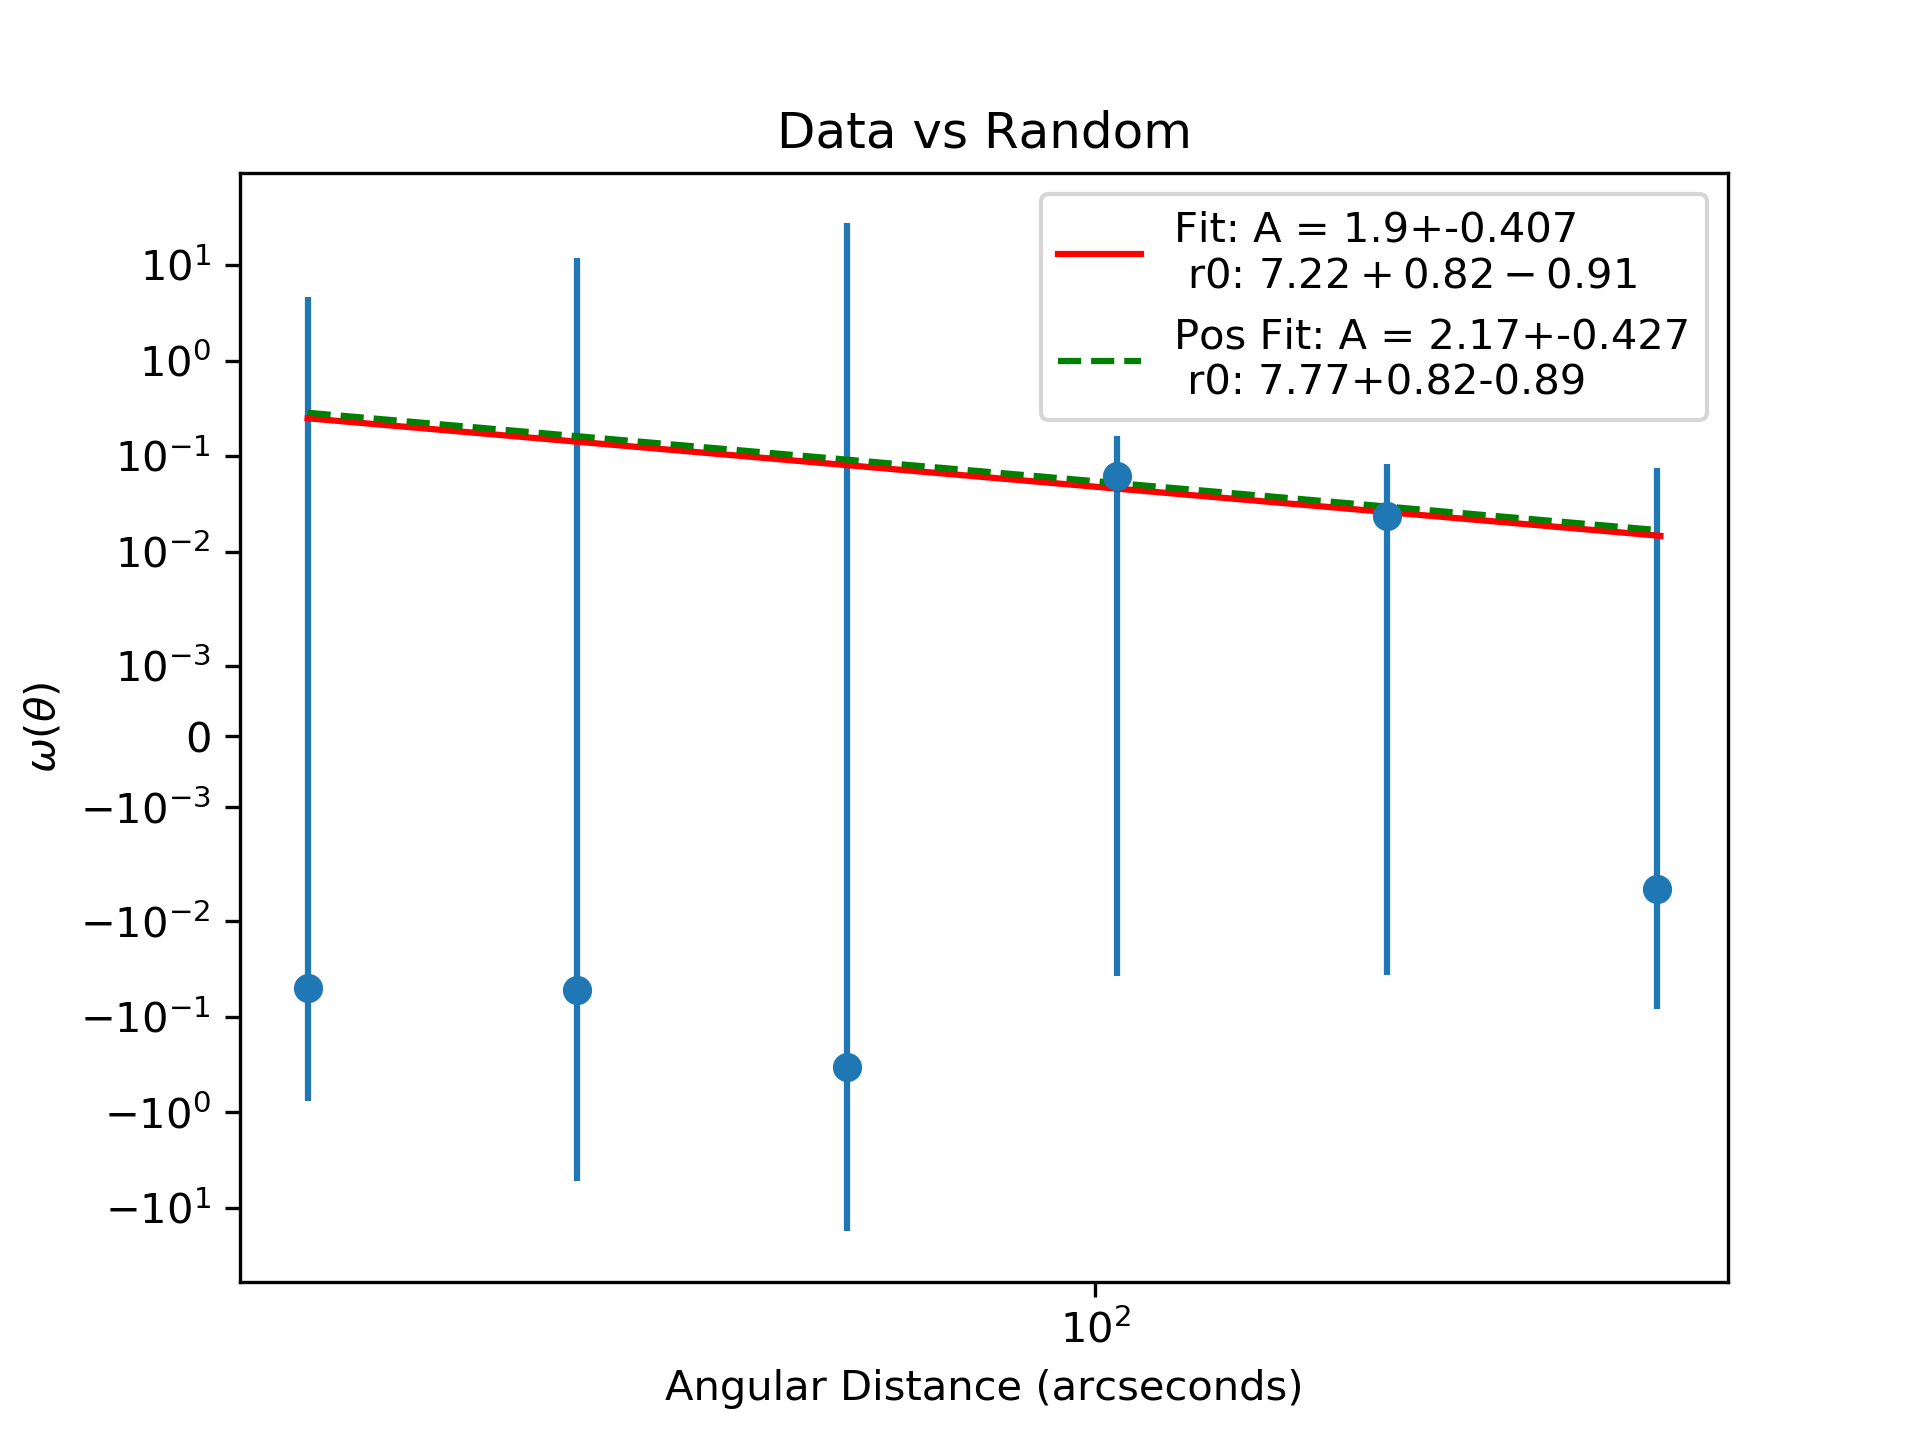
\includegraphics[width=90mm]{clustering_two/Data_vs_Random_10000_bin6_sn0_6_NFalse.png}
\caption{Angular correlation function for 6 bins for the chosen fidelity cut of 0.6. Red is the fit $\omega(\theta) = A\theta^{-0.8}$ to all the bins, while the green line is the fit to only the positive bins. This is the final binning used for the analysis. }
\label{fig:Angular_binnings}
\end{figure}

%3. Explain how the error bars were computed.

The errors were computed through poisson 

%4. Then put what you wrote: Once the angular correlation function is found...angular correlations [7].
%Explain that you fit for all, and then for only positive values.

Once the angular correlation function is found, a power-law model is fitted following $$\omega(\theta) = A\theta^{-\beta} $$ where $\beta$ = 0.8, a value used for many other galaxy angular correlations \cite{hickox2011clustering}. The data was fitted twice, once for all the binned data, and once fitting only to the bins with positive values.

%\subsection{Obtaining $r_0$ and $\gamma$}

%5. Then put the section 3.2.2 until the part where you describe all the equations to compute r0 and gamma. Also here explain that you used the CO z distribution, and the gaussian fit to it. Then report the r0 and gamma values that you measured. And mention somewhere that you have low statistcs.

Two equations are used to convert the $A$ and $\beta$ to real-space $r_0$ and $\gamma$, 

$$ \gamma = \beta + 1 $$ and $$ A = H_{\gamma}\frac{\int_{0}^{\inf} (dN_1/dz)(dN_2/dz)E_z\chi^{1 - \gamma} dz}{[\int_{0}^{\inf} (dN_1/dz)dz][\int_{0}^{\inf} (dN_2/dz)dz]}r_0^{\gamma}$$

where $H_{\gamma} = \Gamma(0.5)\Gamma(0.5[\gamma -1])\Gamma(0.5\gamma)$, with $\Gamma$ being the gamma function, $\chi$ the radial comoving distance, $dN_{1,2}/dz$ are the redshift distributions of the samples, where in the case of autocorrelation are equal to each other, and $E_z = H_z/c = dz/d\chi$ \cite{hickox2011clustering}. The Hubble parameter $H_z$ can be found from
$$H_z^2 = H_0^2[\Omega_m(1+z)^3 + \Omega_{\lambda}]$$ \cite{hickox2011clustering}.

For this analysis, a gaussian was fitted to the CO line candidate's redshift distribution and used as the redshift distribution for $dN_{1,2}/dz$. Because there are only 35 line candidates in the catalog, the clustering measurements are quite noisy. 

\begin{figure}[!tbp]
% explain how bins can be negative and what this means for fitting only positive bins
% Bins can be negative through.... 0, so not negative I guess? 
\centering 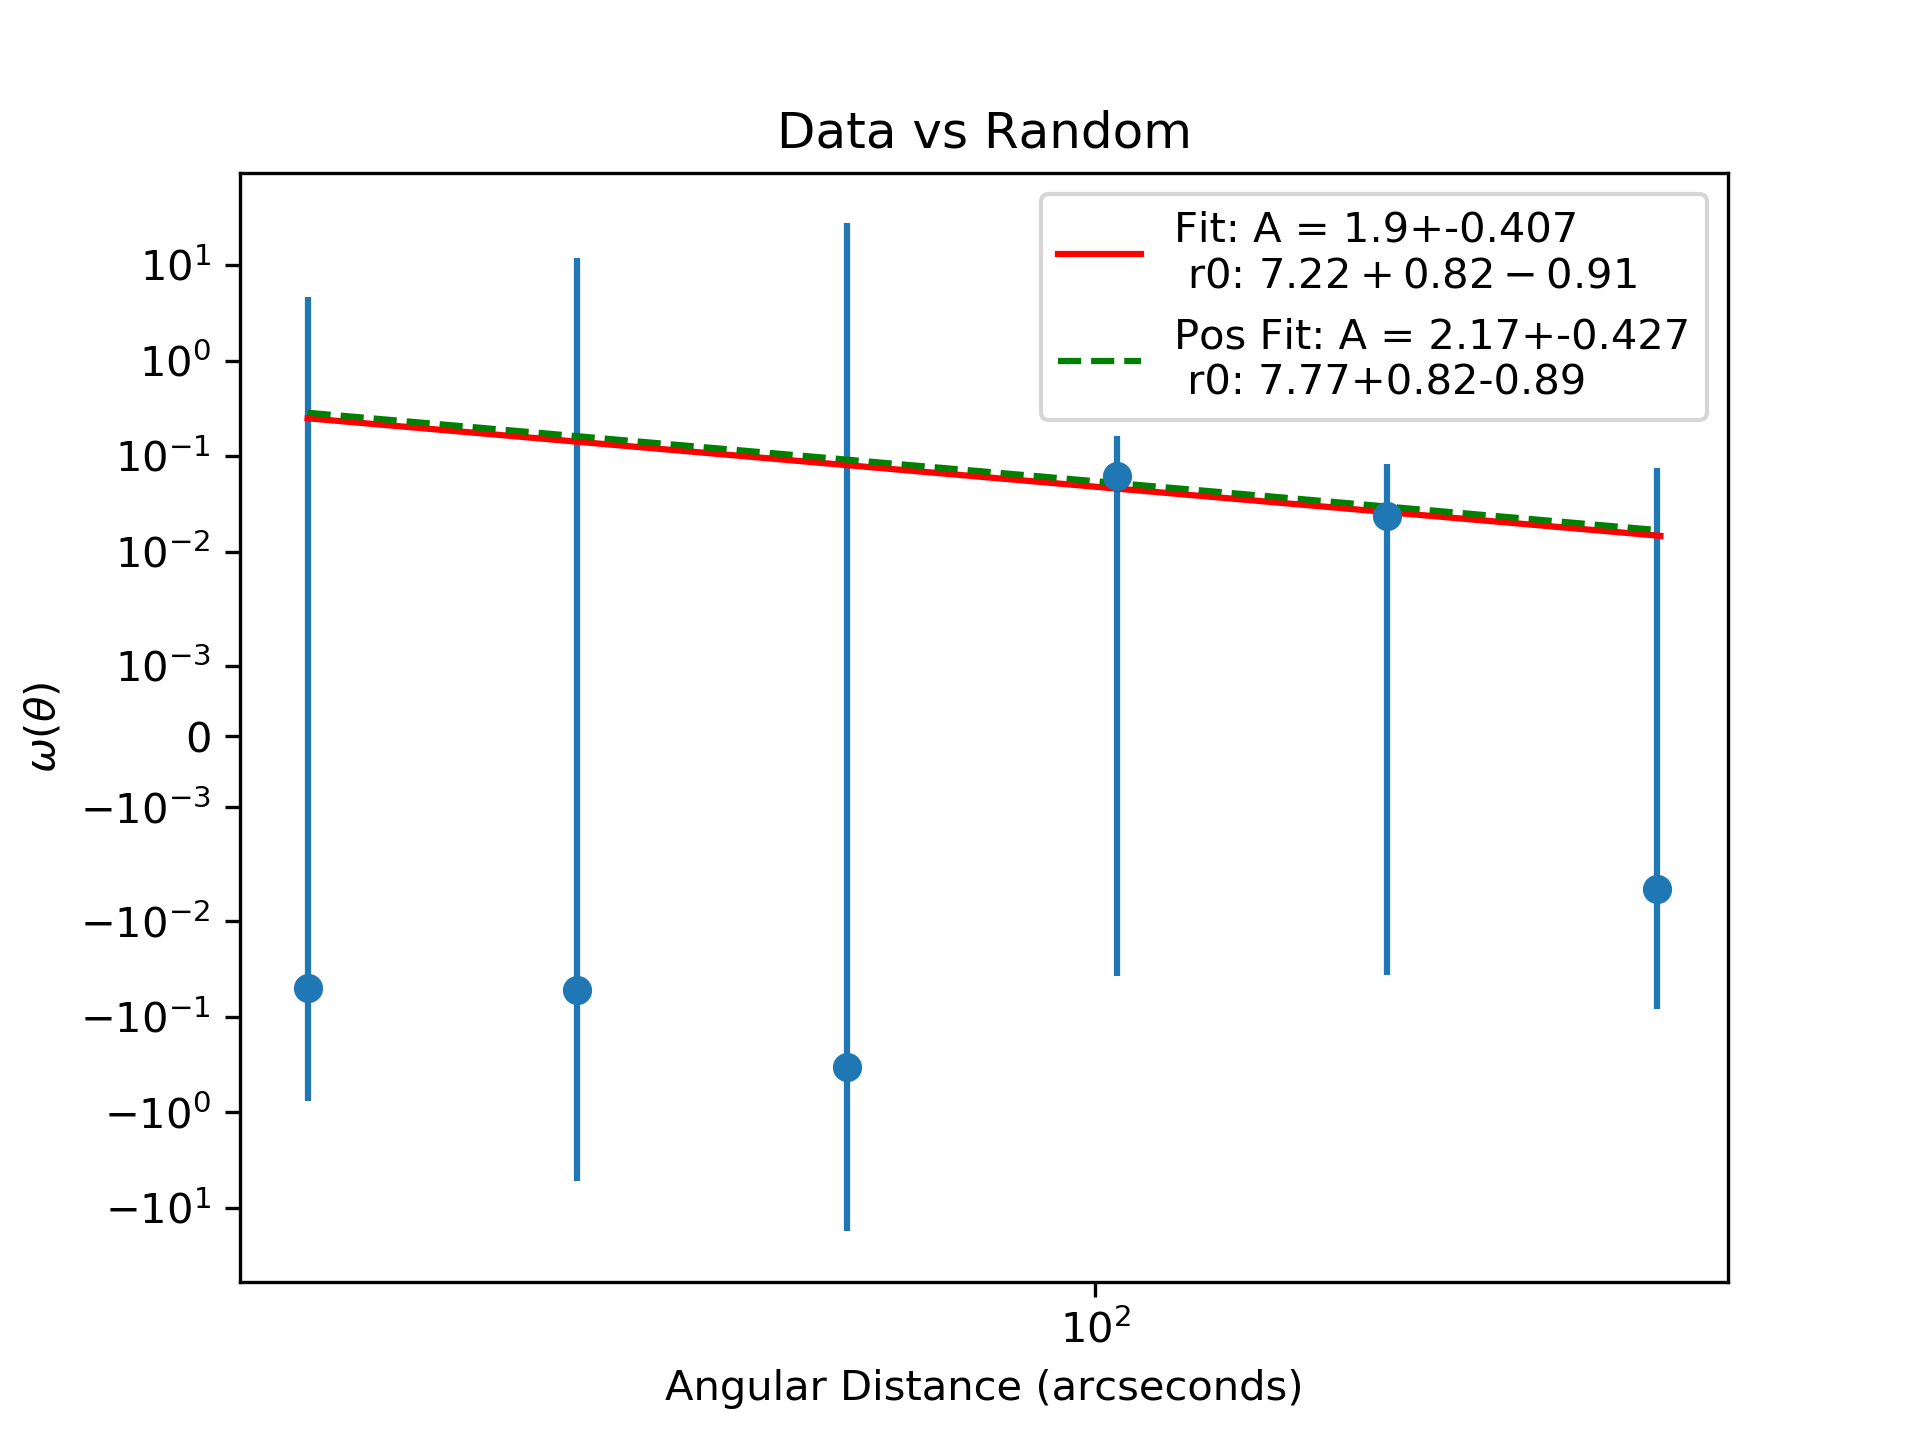
\includegraphics[width=90mm]{clustering_two/Data_vs_Random_10000_bin6_sn0_6_NFalse.png}
\caption{Angular correlation function for 6 bins for the chosen fidelity cut of 0.6. Red is the fit $\omega(\theta) = A\theta^{-0.8}$ to all the bins, while the green line is the fit to only the positive bins. This is the final binning used for the analysis. }
\label{fig:Angular_binnings}
\end{figure}

[FINAL r0 and Gamma]

%6. Then put a discussion section, and comment about if the r0 values that you got is higher or lower to other populations (as you can see in Fig. 3.1). Then say that you did the same procedure for other fidelity cuts to compare, and show your 4panel plot and comment about the fact that signal goes up with fidelity.

\section{Discussion}

% Add more about the effects of binning, negative/0 values 
The clustering results do show that there is a larger $r_0$ as the fidelity cut becomes higher, suggesting that there are real sources in the sample. On the other hand, the clustering measurement is still very noisy and future work will be required to get a better final clustering measurement. The current measurement for $r_0$ seems to depend greatly on the number of bins chosen. 

In comparison to previous results, the $r_0$ of the CO emitters here are quite similar to the values for the SMGs found in \cite{10.1111/j.1365-2966.2011.20303.x}.

As can be seen in Fig. \ref{fig:Angular_correlation}, as the fidelity increases, $A$ increases as well. When converted to $r_0$, the fidelity cuts result in $r_0$ values of $7.89_{-7.89}^{+5.83}$ for fidelity $>$ 0.7, $7.22_{-0.9}^{+0.83}$ for fidelity $>$ 0.6, $0.0_{-0.0}^{+4.03}$ for fidelity $>$ 0.5, and $r_0 = 0.0_{-0.0}^{+0.0}$ for fidelity $>$ 0.4, as the $A$ value is always negative.

As a comparison, the two point correlation function was also computed for other fidelity cuts. The redshift distribution was taken from the CO redshifts of the lines, and the calculations were calculated over the range z = 1.5 to 3.5, as this is the range where most of the CO candidates seem to lie. To calculate $dN_{1,2}/dz$, the redshift distribution of the CO lines was fitted with a Gaussian, and the integral was taken over the Gaussian fit. The angular correlation function was computed over the range of 8.39 to 582.10 arcseconds, using logarithmically spaced bins. 

To calculate the errors on $\omega(\theta)$ the method from \cite{1986ApJ...303..336G} is used. The error bars are computed using possion errors for small statistics \cite{1986ApJ...303..336G}.

% Random points: 582.10 arcseconds, DD points, 516 arcseconds

\begin{figure}[tbp]
% Expand axis to show bottom of points, need to show fit for the red values
% Use Symlog to plot it then, will keep negative values and such
\centering 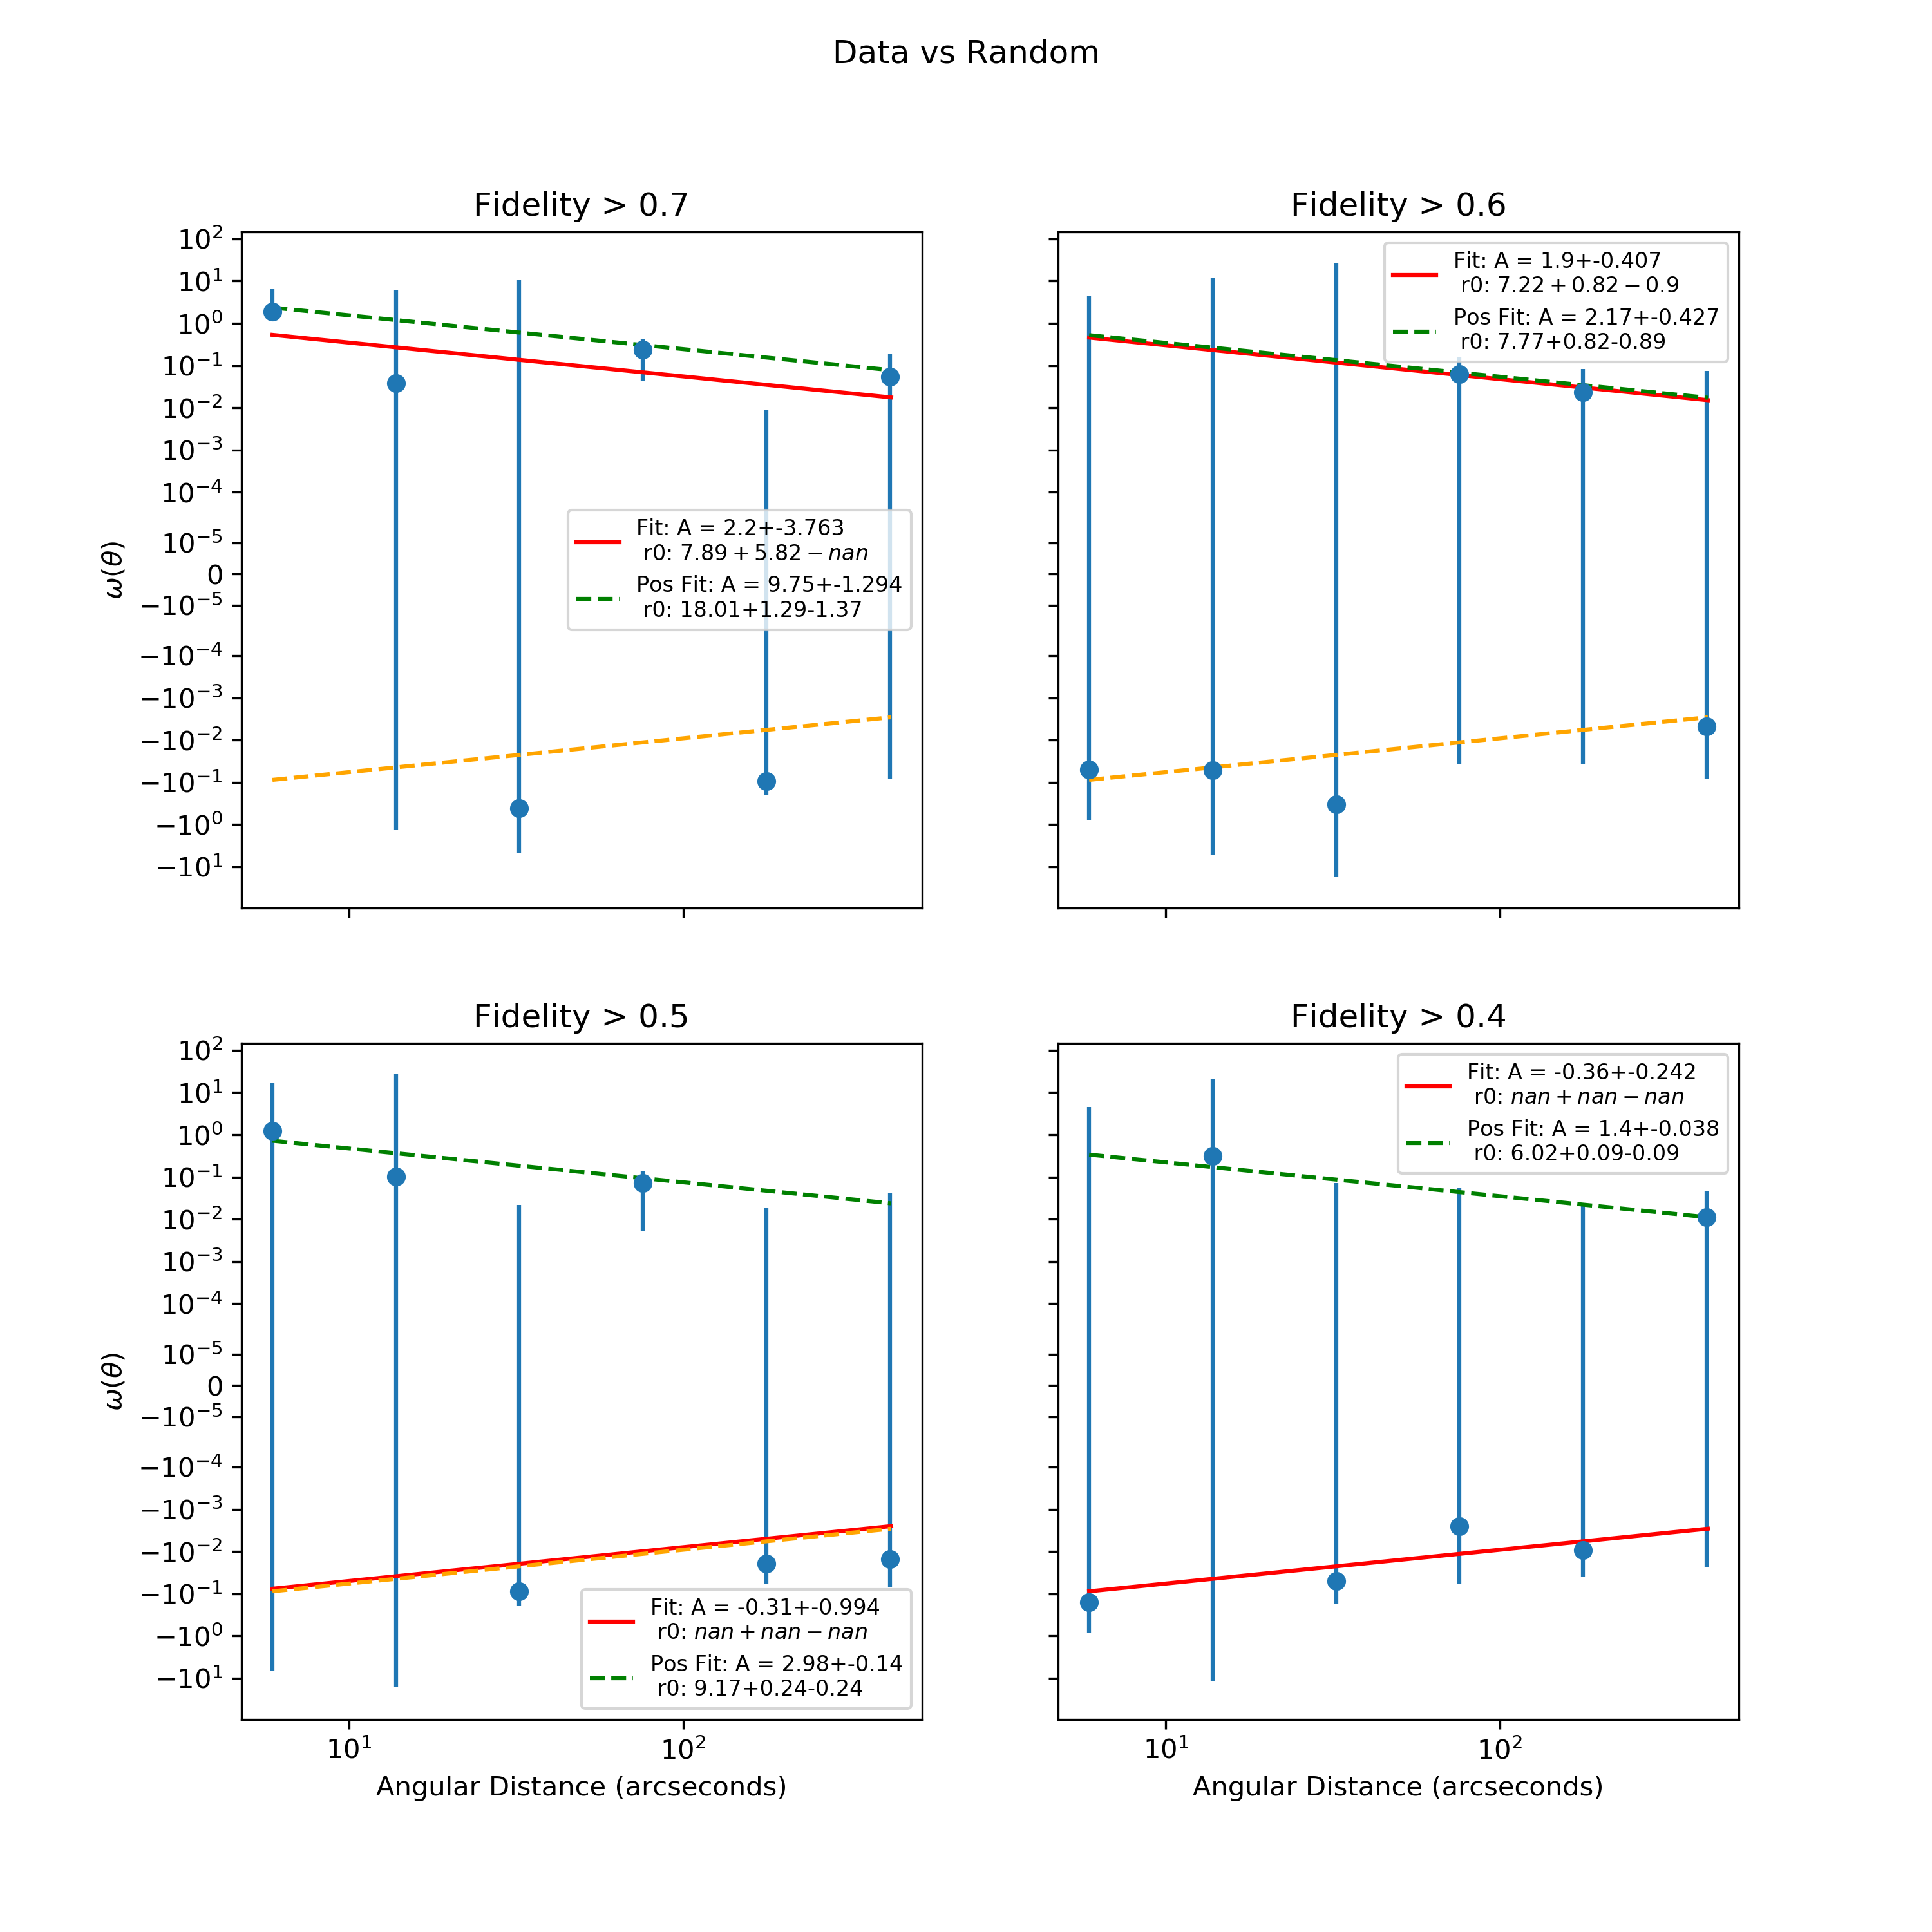
\includegraphics[width=120mm]{clustering_two/Log_4Panel_Data_Vs_Random_bin6_NFalse_Num10000.png}
\caption{Angular correlation function for various fidelity cuts. The bins increase logarithmically from 8.39 arcsecs to 582.10 arcseconds. The red lines are from fitting $\omega(\theta) = A\theta^{-0.8} $ to all of the bins. The green dashed line is from fitting that same equation only to bins that had a positive value. The yellow dashed line is the fit from the fidelity $>$ 0.4 catalog. As the fidelity goes up, the $A$ value increases as well, indicating stronger clustering. The few line candidates means that the results are quite noisy, and are sensitive to the bins chosen.}
\label{fig:Angular_correlation}
\end{figure}

Besides the different fidelity cuts, different distance binnings also are included to study their effects on the final $r_0$ results. The results seem to be very dependent on the binning. While the values for the only positively fitted bins does not change dramatically as the binning changes, the number of bins does make a large difference in the final $A$, and therefore $r_0$ values, as can be seen in Figures \ref{fig:Angular_bin_8} and \ref{fig:Angular_bin_5} in comparison to Fig. \ref{fig:Angular_binnings}.

\begin{figure}[!tbp]
\centering 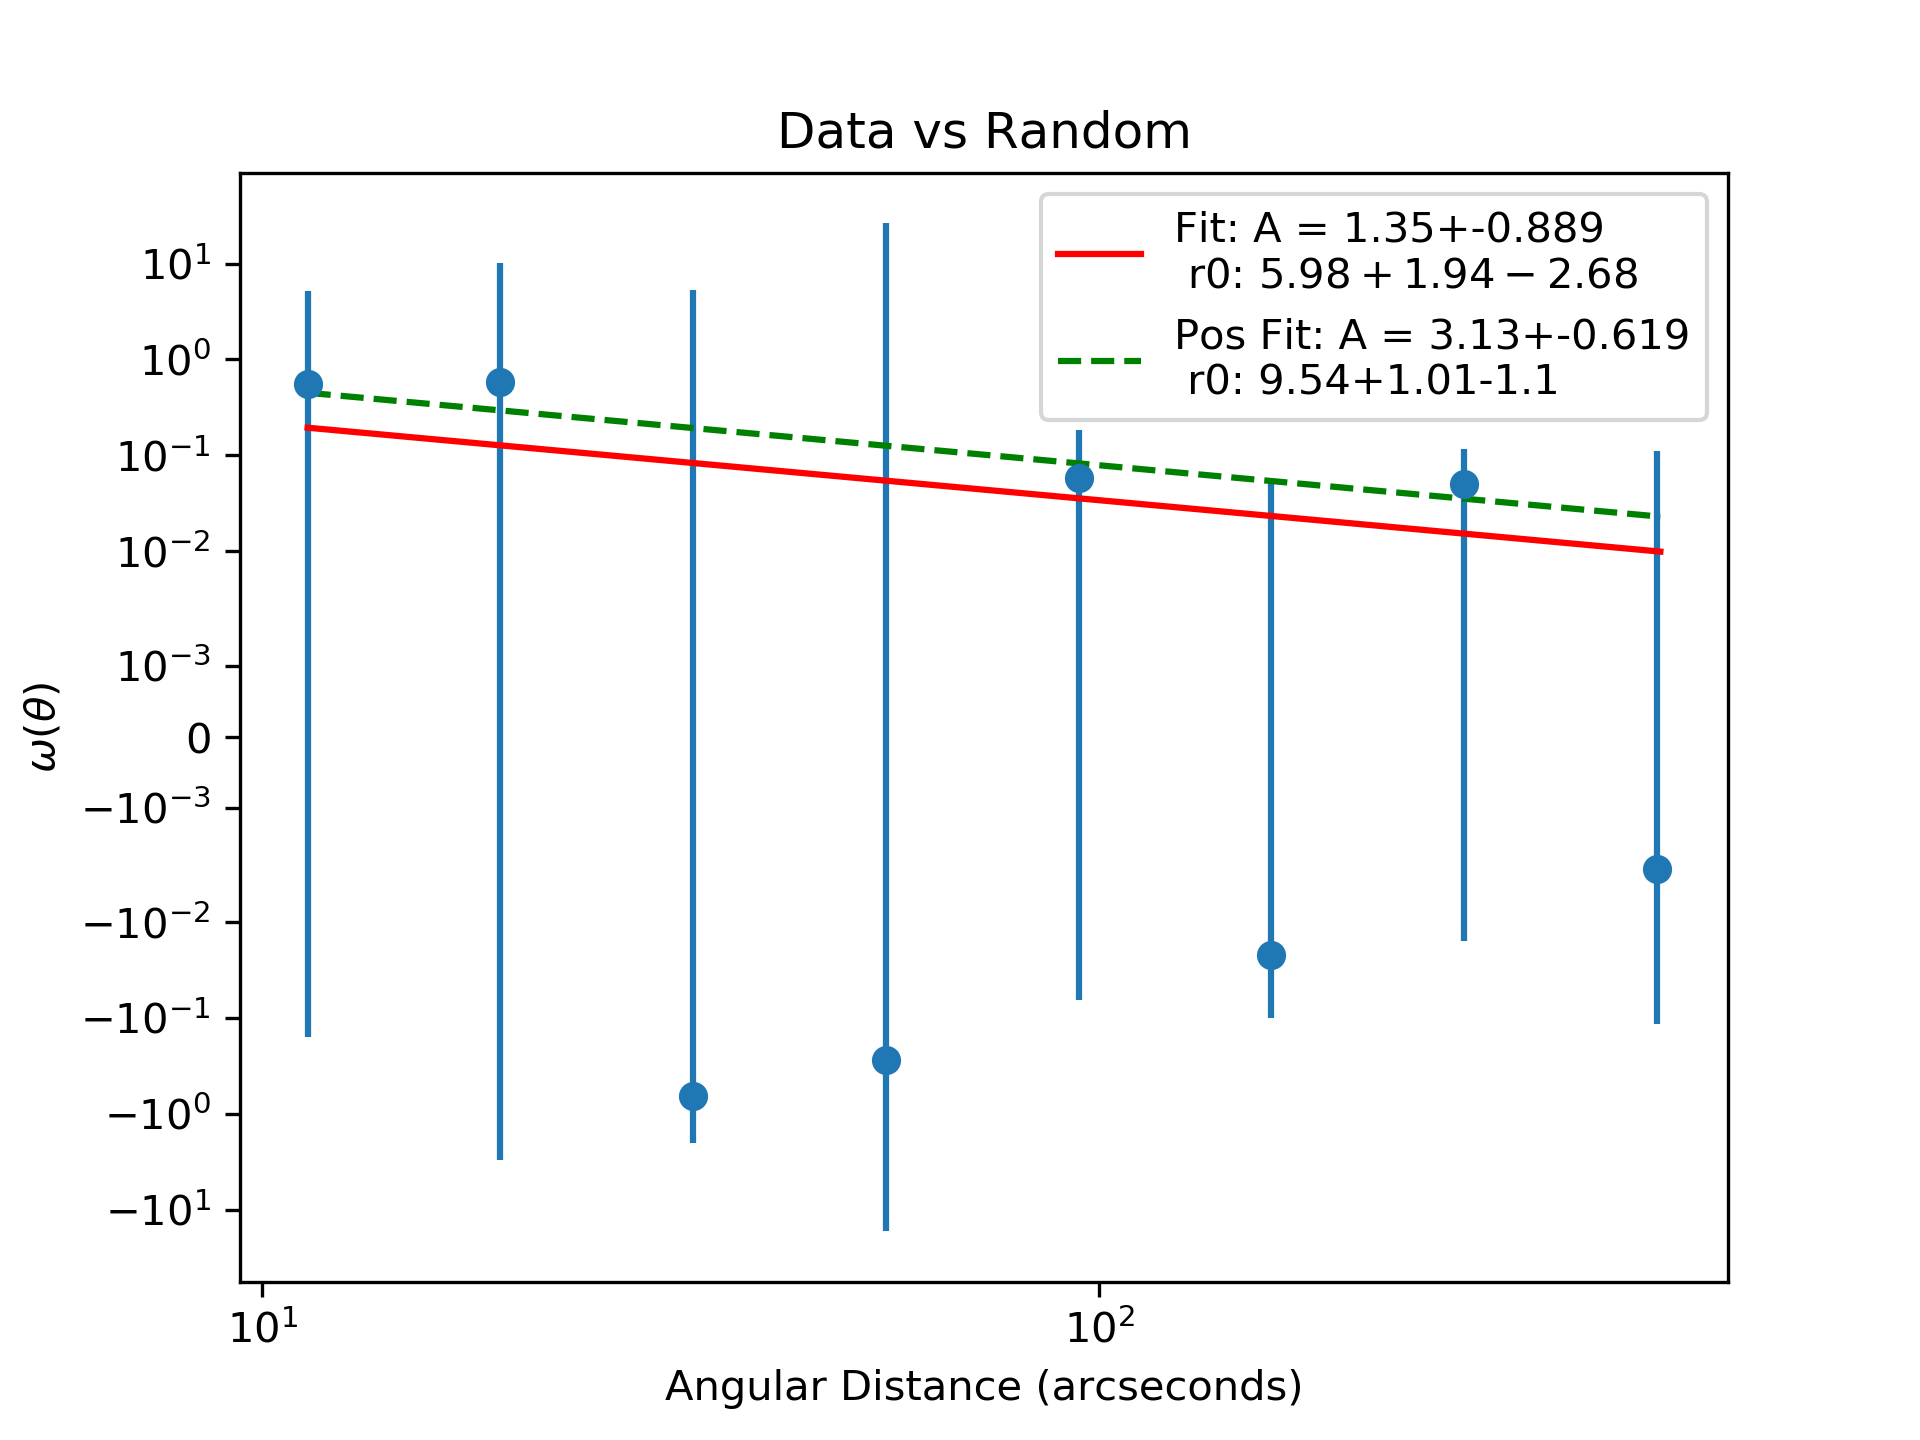
\includegraphics[width=90mm]{clustering_two/Data_vs_Random_10000_bin8_sn0_6_NFalse.png}
\caption{Angular correlation function for 8 bins  for fidelity $>$ 0.6. In this case, an increase in the number of bins decreases the $r_0$ value, although it is still consistent with the original $r_0$ value.}
\label{fig:Angular_bin_8}
\end{figure}

\begin{figure}[!tbp]
\centering 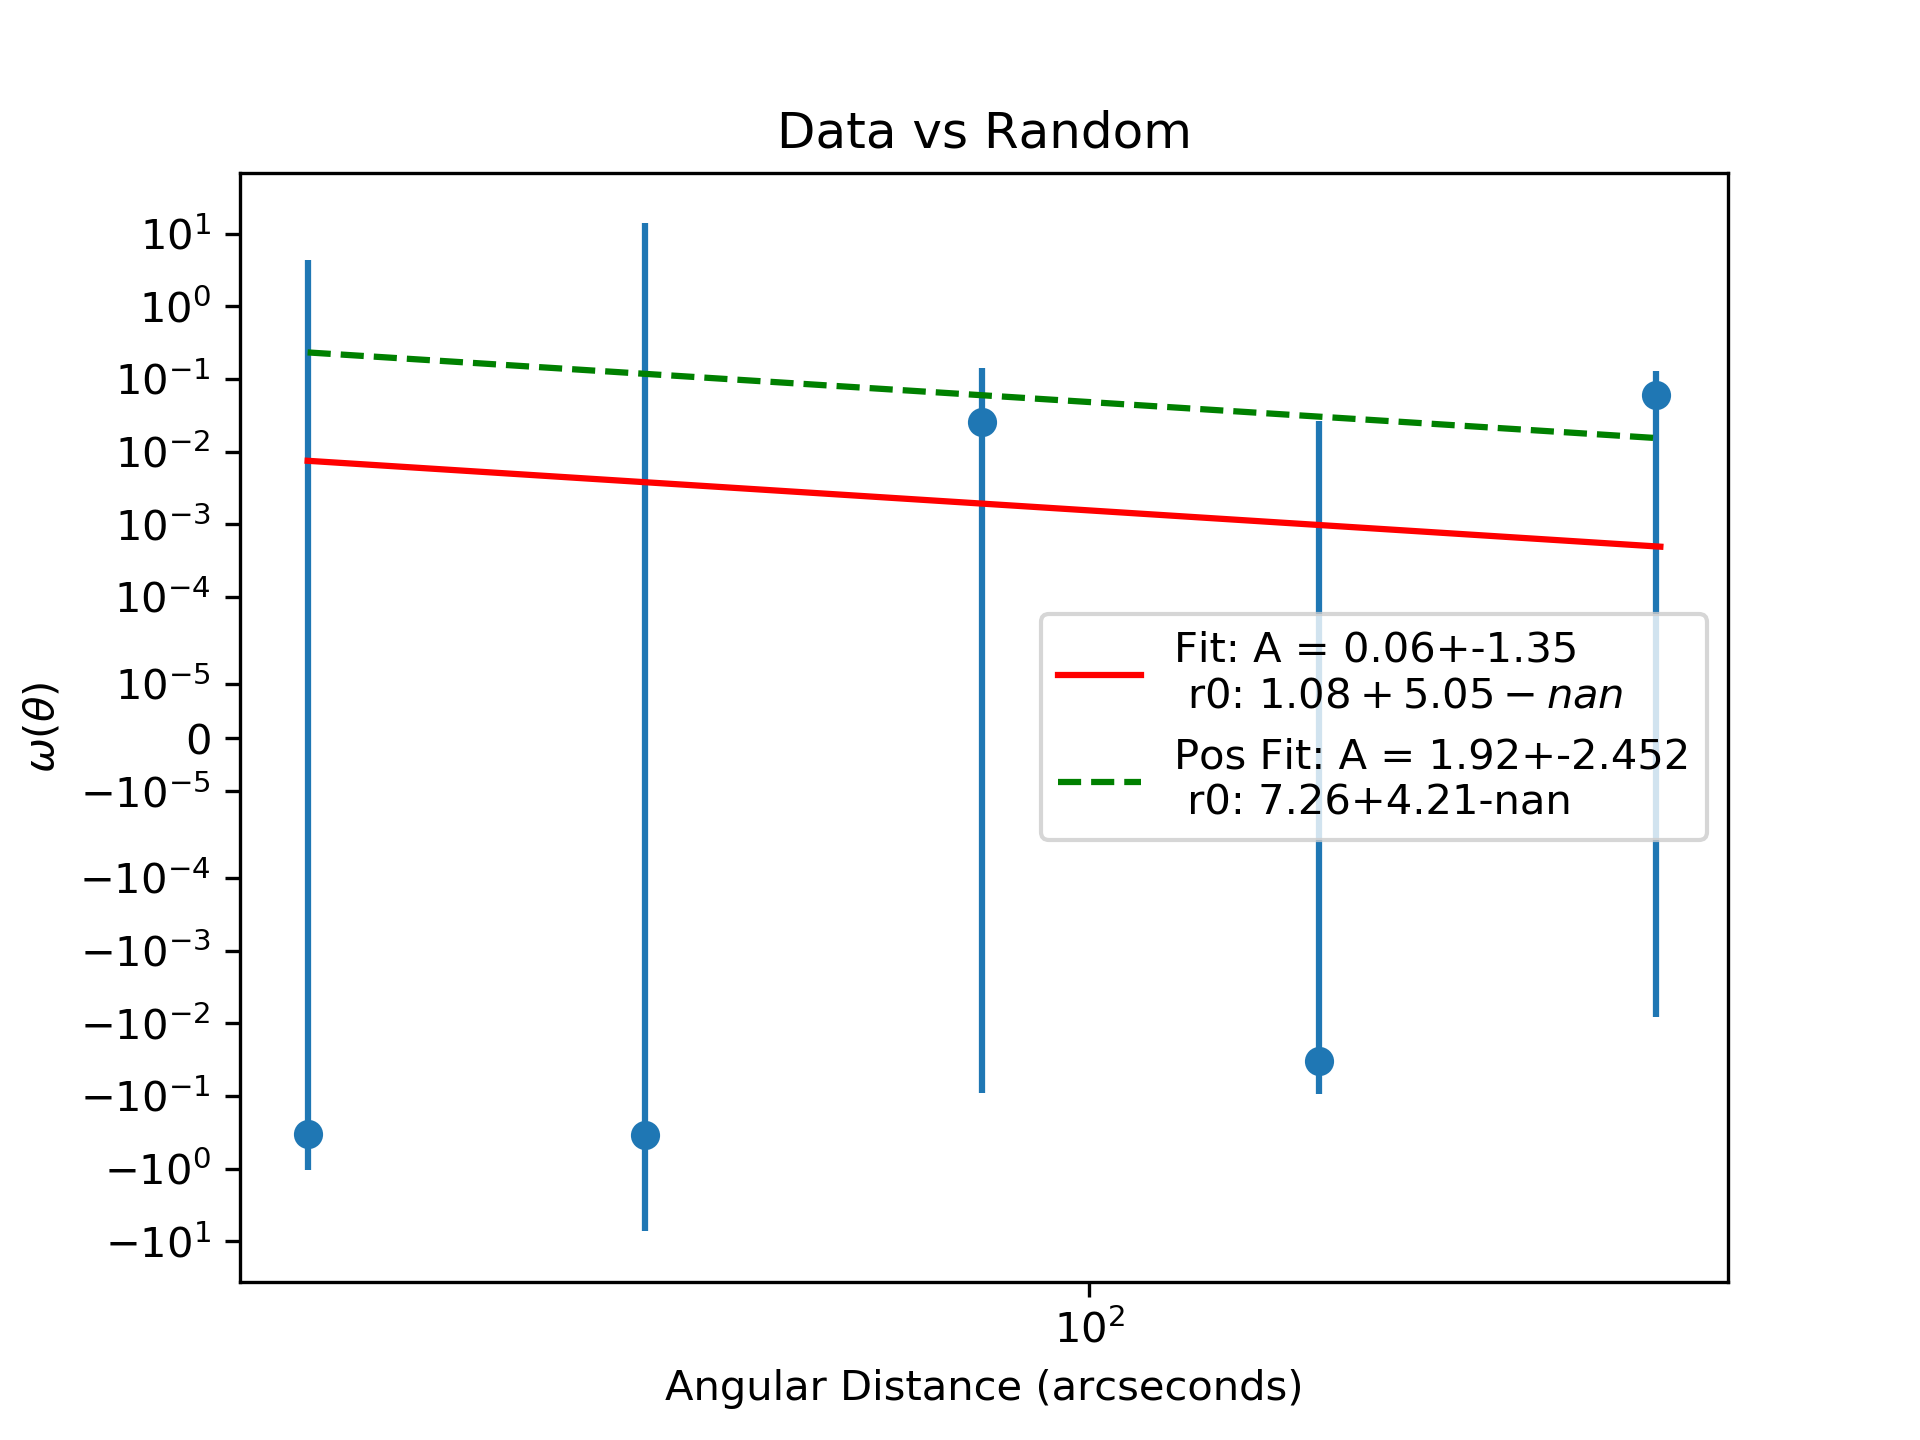
\includegraphics[width=90mm]{clustering_two/Data_vs_Random_10000_bin5_sn0_6_NFalse.png}
\caption{Angular correlation function for 5 bins for fidelity $>$ 0.6. In this case, decreasing the number of bins also decreases the $r_0$ value, which are not consistent with the $r_0$ found originally.}
\label{fig:Angular_bin_5}
\end{figure}


